\documentclass[
	a4paper,
	oneside,
	BCOR = 10mm,
	DIV = 12,
	12pt,
	headings = normal,
]{scrartcl}

%%% Length calculations
\usepackage{calc}
%%%

%%% Support for color
\usepackage{xcolor}
\definecolor{lightblue}{HTML}{03A9F4}
\definecolor{red}{HTML}{F44336}
%%%

%%% Including graphics
\usepackage{graphicx}
%%%

%%% Font selection
\usepackage{fontspec}

\setromanfont{STIX Two Text}[
	SmallCapsFeatures = {LetterSpace = 8},
]

\setsansfont{IBM Plex Sans}[
	Scale = MatchUppercase,
]

\setmonofont{IBM Plex Mono}[
	Scale = MatchUppercase,
]
%%%

%%% Math typesetting
\usepackage{amsmath}

\usepackage{unicode-math}
\setmathfont{STIX Two Math}
%%%

%%% List settings
\usepackage{enumitem}
\setlist[enumerate]{
	label*      = {\arabic*.},
	leftmargin  = *,
	labelindent = \parindent,
	topsep      = 1\baselineskip,
	parsep      = 0\baselineskip,
	itemsep     = 1\baselineskip,
}

\setlist[itemize]{
	label*      = {—},
	leftmargin  = *,
	labelindent = \parindent,
	topsep      = 1\baselineskip,
	parsep      = 0\baselineskip,
	itemsep     = 1\baselineskip,
}

\setlist[description]{
	font        = {\rmfamily\upshape\bfseries},
	topsep      = 1\baselineskip,
	parsep      = 0\baselineskip,
	itemsep     = 0\baselineskip,
}

%%%

%%% Structural elements typesetting
\setkomafont{pagenumber}{\rmfamily}
\setkomafont{disposition}{\rmfamily\bfseries}

% Sectioning
\RedeclareSectionCommand[
	beforeskip = -1\baselineskip,
	afterskip  = 1\baselineskip,
	font       = {\normalsize\bfseries\scshape},
]{section}

\RedeclareSectionCommand[
	beforeskip = -1\baselineskip,
	afterskip  = 1\baselineskip,
	font       = {\normalsize\bfseries\itshape},
]{subsection}

\RedeclareSectionCommand[
	beforeskip = -1\baselineskip,
	afterskip  = 1\baselineskip,
	font       = {\normalsize\bfseries},
]{subsubsection}

\RedeclareSectionCommand[
	beforeskip = -1\baselineskip,
	afterskip  = -0.5em,
	font       = {\normalsize\mdseries\scshape\addfontfeatures{Letters = {UppercaseSmallCaps}}},
]{paragraph}
%%%

%%% Typographic enhancements
\usepackage{microtype}
%%%

%%% Language-specific settings
\usepackage{polyglossia}
\setmainlanguage{ukrainian}
\setotherlanguages{english}
%%%

%%% Captions
\usepackage{caption}
\usepackage{subcaption}

%\DeclareCaptionLabelFormat{closing}{#2)}
%\captionsetup[subtable]{labelformat = closing}

%\captionsetup[subfigure]{labelformat = closing}

\captionsetup[table]{
	aboveskip = 0\baselineskip,
	belowskip = 0\baselineskip,
}

\captionsetup[figure]{
	aboveskip = 1\baselineskip,
	belowskip = 0\baselineskip,
}

\captionsetup[subfigure]{
	labelformat = simple,
	labelformat = brace,
}
%%%

%%% Hyphenated ragged typesetting
\usepackage{ragged2e}
%%%

%%% Table typesetting
\usepackage{booktabs}
\usepackage{longtable}

\usepackage{multirow}

\usepackage{array}
\newcolumntype{v}[1]{>{\RaggedRight\arraybackslash\hspace{0pt}}p{#1}}
\newcolumntype{b}[1]{>{\Centering\arraybackslash\hspace{0pt}}p{#1}}
\newcolumntype{n}[1]{>{\RaggedLeft\arraybackslash\hspace{0pt}}p{#1}}
%%%

%%% Drawing
\usepackage{tikz}
\usepackage{tikzscale}
\usetikzlibrary{positioning}
\usetikzlibrary{arrows.meta} % Stealth arrow tips
%%%

%%% SI units typesetting
\usepackage{siunitx}
\sisetup{
	output-decimal-marker = {,},
	exponent-product      = {\cdot},
	inter-unit-product    = \ensuremath{{} \cdot {}},
	per-mode              = symbol,
}
%%%

%%% Links and hyperreferences
\usepackage{hyperref}
\hypersetup{
	bookmarksnumbered = true,
	colorlinks      = false,
	linkbordercolor = red,
	urlbordercolor  = lightblue,
	pdfborderstyle  = {/S/U/W 1.5},
}
%%%

%%% Length adjustments
% Set baselineskip, default is 14.5 pt
\linespread{1.068966} % ~15.5 pt
\setlength{\emergencystretch}{1em}
\setlength{\parindent}{1.5em}
\newlength{\gridunitwidth}
\setlength{\gridunitwidth}{\textwidth / 12}
%%%

%%% Custom commands
\newcommand{\allcaps}[1]{{\addfontfeatures{LetterSpace = 8, Kerning = Off}#1}}
%%%

\begin{document}

\begin{titlepage}
		\begin{center}
			Міністерство освіти і науки України\\
			Національний авіаційний університет\\
			Навчально-науковий інститут комп'ютерних інформаційних технологій\\
			Кафедра комп'ютеризованих систем управління

			\vspace{\fill}
				Лабораторна робота №2.1\\
				з дисципліни «Телекомунікаційні~технології комп'ютерних~мереж»\\
				на тему «Моделювання передавальної частини цифрової системи зв'язку»

			\vspace{\fill}

			\begin{flushright}
				Виконав:\\
				студент \allcaps{ННІКІТ}\\
				групи СП-325\\
				Клокун В.\,Д.\\
				Перевірив:\\
				Пушкін Ю.\,О.
			\end{flushright}

			Київ 2018
		\end{center}
	\end{titlepage}

	\section{Мета роботи}
		Вивчення принципів формування сигналу в системах цифрового зв'язку.

	\section{Завдання роботи}
		Опис теоретичної моделі досліджуваної системи передачі даних, створення моделі передавального пристрою цифрової системи зв'язку в \textenglish{Simulink}; моделювання роботи системи при різних початкових умовах; вимір основних параметрів роботи передавальної системи.

	\section{Хід роботи}
		\subsection{Створення моделі}
			Створюємо модель передавальної системи, яка~складається з~генератора випадкових цілих чисел, модулятора, спектрального аналізатора, блоку виділення дійсної і~комплексної частин сигналу та~осцилографа~(рис.~\ref{subfig:01-simulink-tx-model-full}).

			\begin{figure}[!htbp]
				\begin{subfigure}[t]{\textwidth / 2}
					\centering
					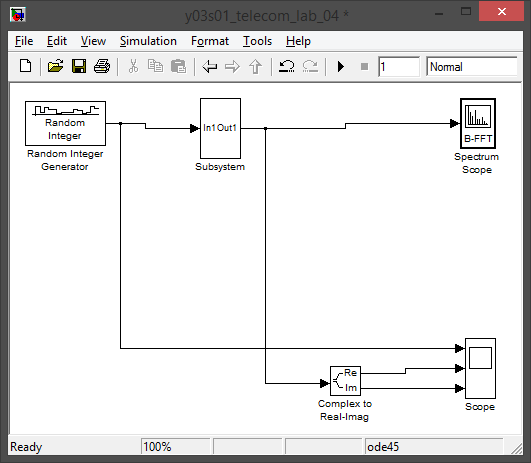
\includegraphics[height = 9\baselineskip]{./assets/y03s01-telecom-lab-04-simulink-full-model.png}
					\caption{}
					\label{subfig:01-simulink-tx-model-full}
				\end{subfigure}%
				\begin{subfigure}[t]{\textwidth / 2}
					\centering
					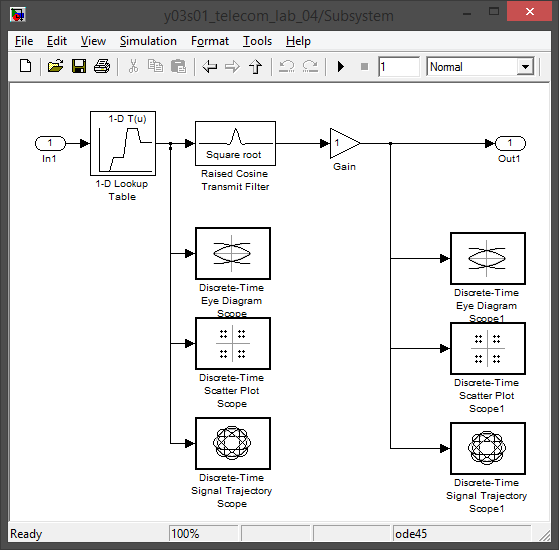
\includegraphics[height = 9\baselineskip]{./assets/y03s01-telecom-lab-04-simulink-tx-model.png}
					\caption{}
					\label{subfig:01-simulink-tx-model-transmitter}
				\end{subfigure}
				\caption{Модель передавальної системи: \subref{subfig:01-simulink-tx-model-full}~— загальний вигляд, \subref{subfig:01-simulink-tx-model-transmitter}~— формувач сигналу}
				\label{fig:01-simulink-tx-model}
			\end{figure}

			В~моделі створюємо підсистему формувача сигналу, який складається з~таблиці істинності, формуючого фільтру з~характеристикою піднесеного косинуса та~підсилювача~(рис.~\ref{subfig:01-simulink-tx-model-transmitter}).

		\subsection{Симуляція роботи створеної моделі системи передачі даних}
			Для виконання завдання роботи виконуємо симуляцію з заданими коефіцієнтами скруглення~— $0.0, 0.2, 0.4, 0.6, 0.8, 1.0$.

			\clearpage
			\subsubsection{Симуляція з коефіцієнтом скруглення~0.0}
				Встановлюємо коефіцієнт скруглення фільтра~$0.0$ та~запускаємо моделювання, отримаємо результати на~графіках~(рис.~\ref{fig:rolloff-0p0-spectrum-scope}, \ref{fig:rolloff-0p0-scope}, \ref{fig:rolloff-0p0-plots}).

				\begin{figure}[!htbp]
					\begin{minipage}[t]{0.5\textwidth - 0.5em}
						\centering
						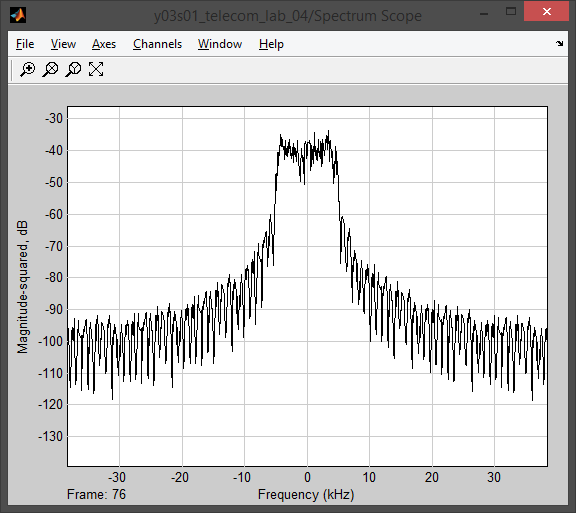
\includegraphics[height = 8\baselineskip]{../01-solution/rolloff-0p0-spectrum-scope.png}
						\caption{Спектр сигналу, що формується}
						\label{fig:rolloff-0p0-spectrum-scope}
					\end{minipage}\hspace{1em}%
					\begin{minipage}[t]{0.5\textwidth - 0.5em}
						\centering
						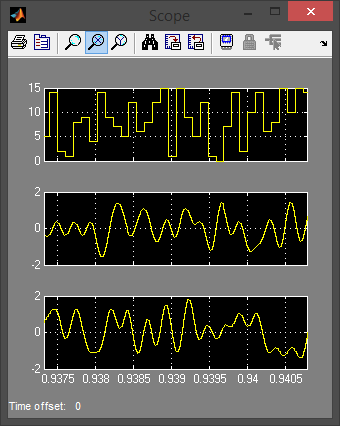
\includegraphics[height = 8\baselineskip]{../01-solution/rolloff-0p0-scope.png}
						\caption{Осцилограми шини даних та~комплексної обвідної сформованого сигналу}
						\label{fig:rolloff-0p0-scope}
					\end{minipage}%
				\end{figure}

				\begin{figure}[!htbp]
					\centering
					\begin{subfigure}{\textwidth / 3}
						\centering
						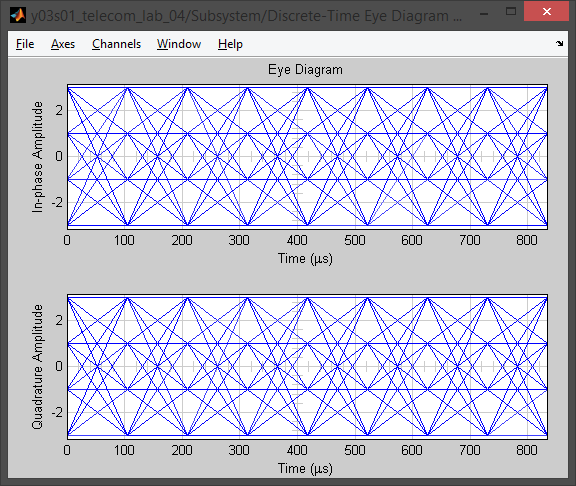
\includegraphics[height = 7\baselineskip]{../01-solution/rolloff-0p0-eye-diag-in.png}
						\caption{}
						\label{subfig:rolloff-0p0-eye-in}
					\end{subfigure}%
					\begin{subfigure}{\textwidth / 3}
						\centering
						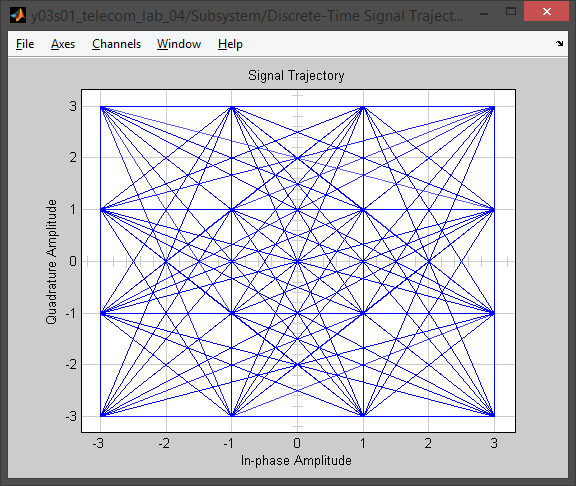
\includegraphics[height = 7\baselineskip]{../01-solution/rolloff-0p0-signal-trajectory-in.png}
						\caption{}
						\label{subfig:rolloff-0p0-signal-trajectory-in}
					\end{subfigure}%
					\begin{subfigure}{\textwidth / 3}
						\centering
						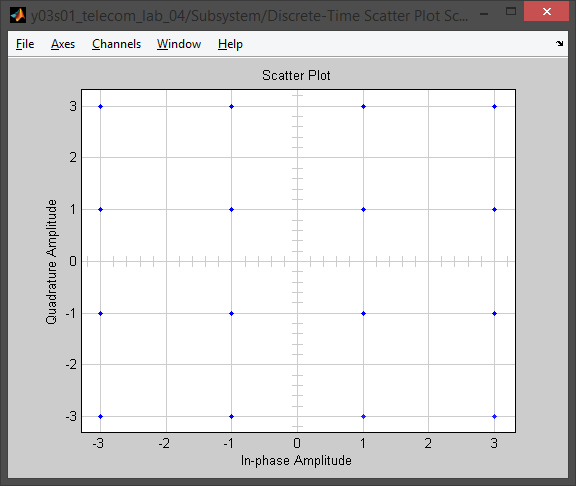
\includegraphics[height = 7\baselineskip]{../01-solution/rolloff-0p0-scatter-plot-in.png}
						\caption{}
						\label{subfig:rolloff-0p0-scatter-plot-in}
					\end{subfigure}
					\begin{subfigure}{\textwidth / 3}
						\centering
						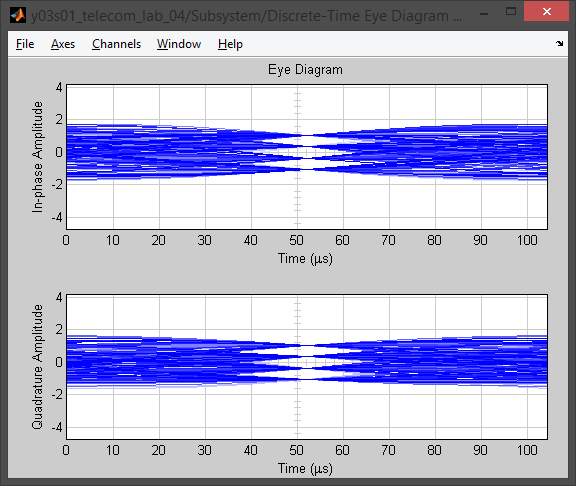
\includegraphics[height = 7\baselineskip]{../01-solution/rolloff-0p0-eye-diag-out.png}
						\caption{}
						\label{subfig:rolloff-0p0-eye-out}
					\end{subfigure}%
					\begin{subfigure}{\textwidth / 3}
						\centering
						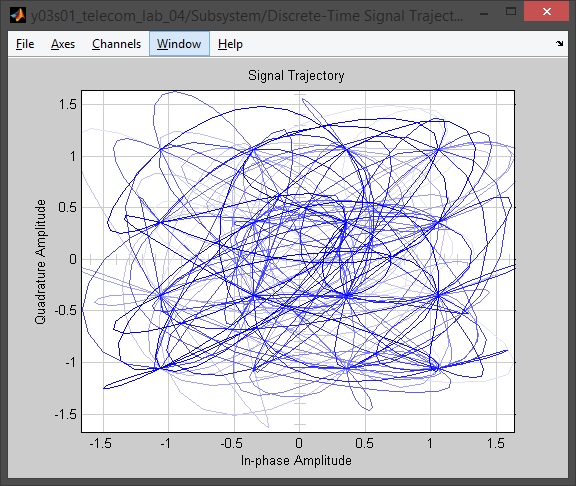
\includegraphics[height = 7\baselineskip]{../01-solution/rolloff-0p0-signal-trajectory-out.png}
						\caption{}
						\label{subfig:rolloff-0p0-signal-trajectory-out}
					\end{subfigure}%
					\begin{subfigure}{\textwidth / 3}
						\centering
						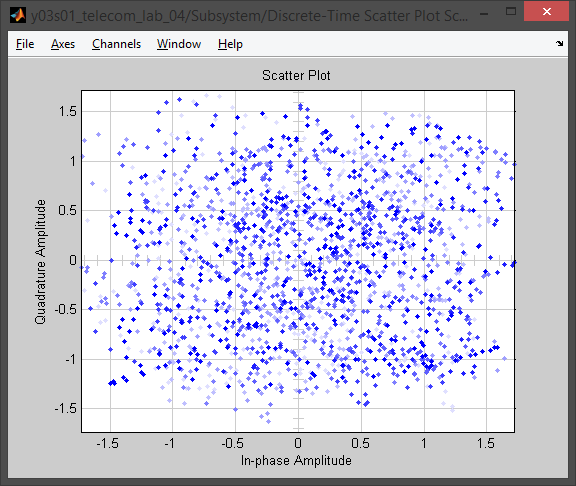
\includegraphics[height = 7\baselineskip]{../01-solution/rolloff-0p0-scatter-plot-out.png}
						\caption{}
						\label{subfig:rolloff-0p0-scatter-plot-out}
					\end{subfigure}%
					\caption{Графіки моделювання для коефіцієнта скруглення~$0.0$: \subref{subfig:rolloff-0p0-eye-in}–\subref{subfig:rolloff-0p0-scatter-plot-in}~— вхідні діаграми (глазкова, траекторії вектора комплексної обвідної, розсіювання відповідно); \subref{subfig:rolloff-0p0-eye-out}–\subref{subfig:rolloff-0p0-scatter-plot-out}~— вихідні діаграми (глазкова, траекторії вектора комплексної обвідної, розсіювання відповідно)}
					\label{fig:rolloff-0p0-plots}
				\end{figure}

			\clearpage
			\subsubsection{Симуляція з коефіцієнтом скруглення~0.2}
				Встановлюємо коефіцієнт скруглення фільтра~$0.2$ та~запускаємо моделювання, отримаємо результати на~графіках~(рис.~\ref{fig:rolloff-0p2-spectrum-scope}, \ref{fig:rolloff-0p2-scope}, \ref{fig:rolloff-0p2-plots}).

				\begin{figure}[!htbp]
					\begin{minipage}[t]{0.5\textwidth - 0.5em}
						\centering
						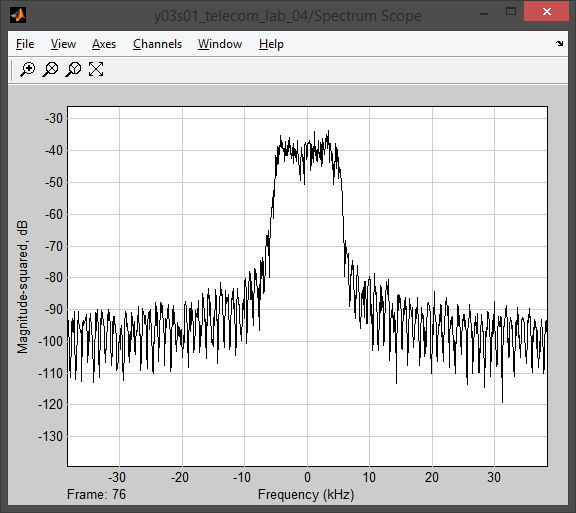
\includegraphics[height = 8\baselineskip]{../01-solution/rolloff-0p2-spectrum-scope.png}
						\caption{Спектр сигналу, що формується}
						\label{fig:rolloff-0p2-spectrum-scope}
					\end{minipage}\hspace{1em}%
					\begin{minipage}[t]{0.5\textwidth - 0.5em}
						\centering
						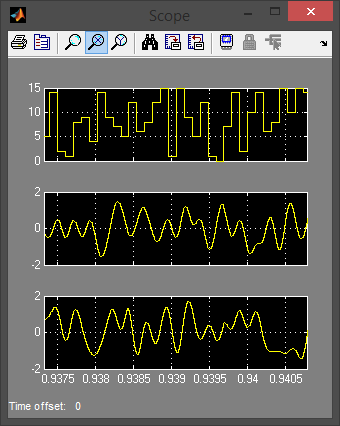
\includegraphics[height = 8\baselineskip]{../01-solution/rolloff-0p2-scope.png}
						\caption{Осцилограми шини даних та~комплексної обвідної сформованого сигналу}
						\label{fig:rolloff-0p2-scope}
					\end{minipage}%
				\end{figure}

				\begin{figure}[!htbp]
					\centering
					\begin{subfigure}{\textwidth / 3}
						\centering
						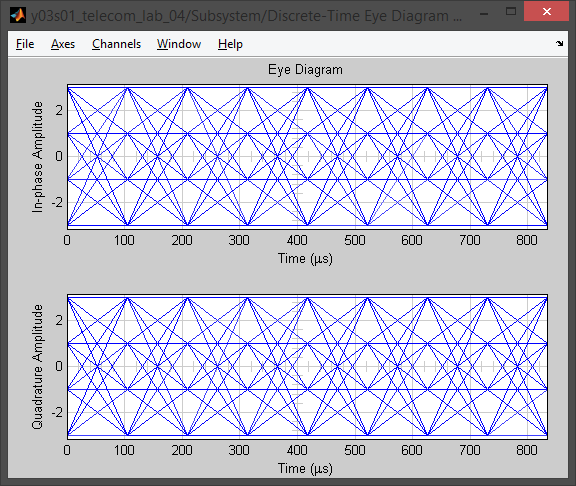
\includegraphics[height = 7\baselineskip]{../01-solution/rolloff-0p2-eye-diag-in.png}
						\caption{}
						\label{subfig:rolloff-0p2-eye-in}
					\end{subfigure}%
					\begin{subfigure}{\textwidth / 3}
						\centering
						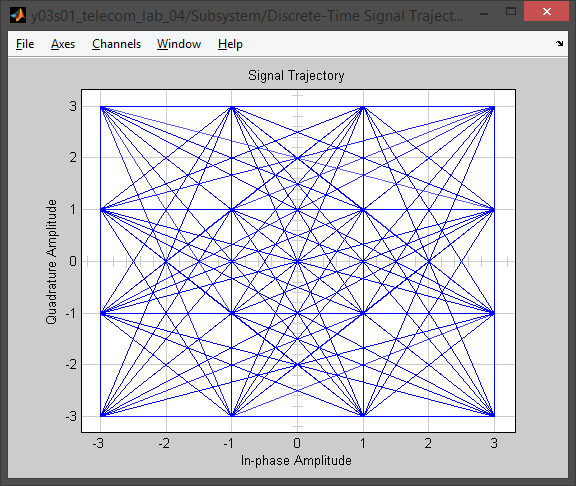
\includegraphics[height = 7\baselineskip]{../01-solution/rolloff-0p2-signal-trajectory-in.png}
						\caption{}
						\label{subfig:rolloff-0p2-signal-trajectory-in}
					\end{subfigure}%
					\begin{subfigure}{\textwidth / 3}
						\centering
						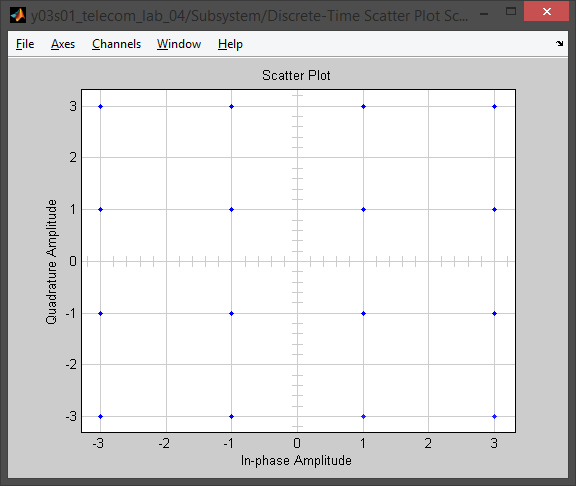
\includegraphics[height = 7\baselineskip]{../01-solution/rolloff-0p2-scatter-plot-in.png}
						\caption{}
						\label{subfig:rolloff-0p2-scatter-plot-in}
					\end{subfigure}
					\begin{subfigure}{\textwidth / 3}
						\centering
						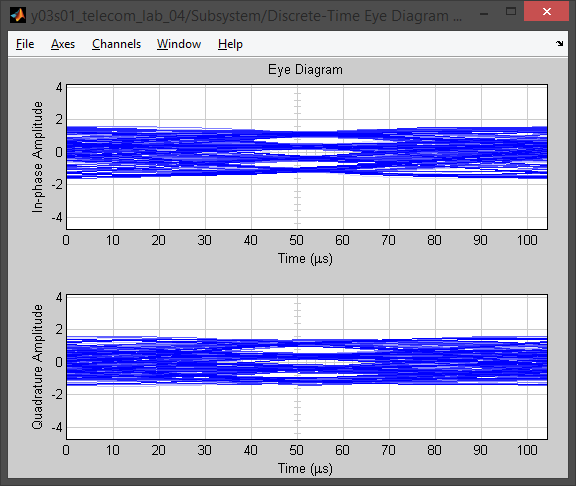
\includegraphics[height = 7\baselineskip]{../01-solution/rolloff-0p2-eye-diag-out.png}
						\caption{}
						\label{subfig:rolloff-0p2-eye-out}
					\end{subfigure}%
					\begin{subfigure}{\textwidth / 3}
						\centering
						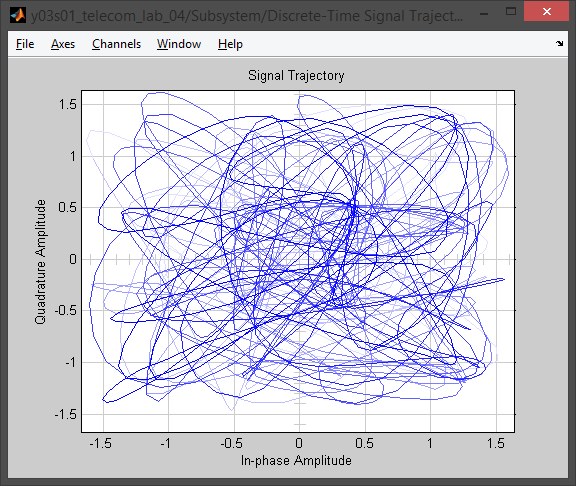
\includegraphics[height = 7\baselineskip]{../01-solution/rolloff-0p2-signal-trajectory-out.png}
						\caption{}
						\label{subfig:rolloff-0p2-signal-trajectory-out}
					\end{subfigure}%
					\begin{subfigure}{\textwidth / 3}
						\centering
						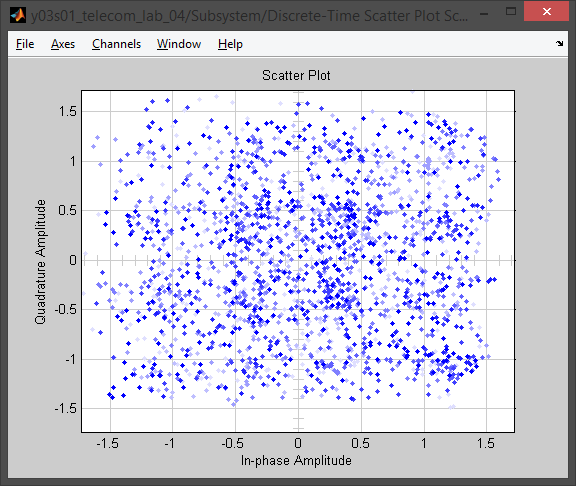
\includegraphics[height = 7\baselineskip]{../01-solution/rolloff-0p2-scatter-plot-out.png}
						\caption{}
						\label{subfig:rolloff-0p2-scatter-plot-out}
					\end{subfigure}%
					\caption{Графіки моделювання для коефіцієнта скруглення~$0.2$: \subref{subfig:rolloff-0p2-eye-in}–\subref{subfig:rolloff-0p2-scatter-plot-in}~— вхідні діаграми (глазкова, траекторії вектора комплексної обвідної, розсіювання відповідно); \subref{subfig:rolloff-0p2-eye-out}–\subref{subfig:rolloff-0p2-scatter-plot-out}~— вихідні діаграми (глазкова, траекторії вектора комплексної обвідної, розсіювання відповідно)}
					\label{fig:rolloff-0p2-plots}
				\end{figure}

			\clearpage
			\subsubsection{Симуляція з коефіцієнтом скруглення~0.4}
				Встановлюємо коефіцієнт скруглення фільтра~$0.4$ та~запускаємо моделювання, отримаємо результати на~графіках~(рис.~\ref{fig:rolloff-0p4-spectrum-scope}, \ref{fig:rolloff-0p4-scope}, \ref{fig:rolloff-0p4-plots}).

				\begin{figure}[!htbp]
					\begin{minipage}[t]{0.5\textwidth - 0.5em}
						\centering
						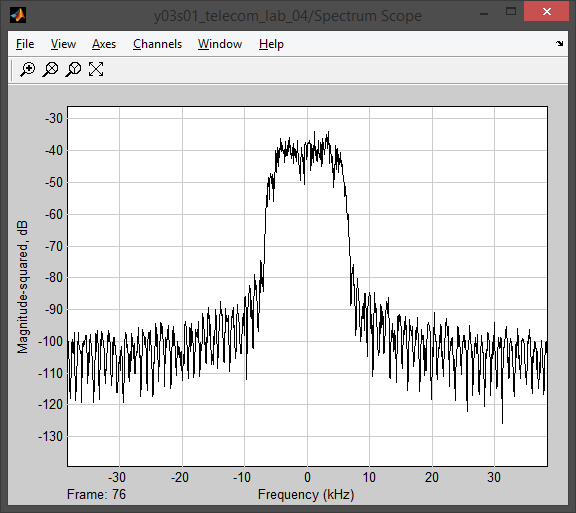
\includegraphics[height = 8\baselineskip]{../01-solution/rolloff-0p4-spectrum-scope.png}
						\caption{Спектр сигналу, що формується}
						\label{fig:rolloff-0p4-spectrum-scope}
					\end{minipage}\hspace{1em}%
					\begin{minipage}[t]{0.5\textwidth - 0.5em}
						\centering
						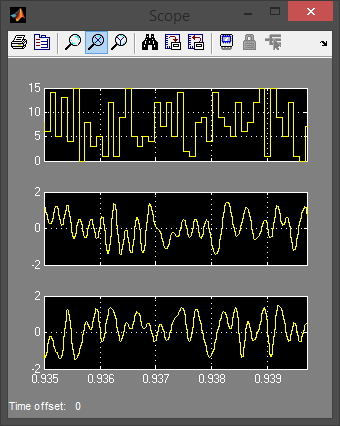
\includegraphics[height = 8\baselineskip]{../01-solution/rolloff-0p4-scope.png}
						\caption{Осцилограми шини даних та~комплексної обвідної сформованого сигналу}
						\label{fig:rolloff-0p4-scope}
					\end{minipage}%
				\end{figure}

				\begin{figure}[!htbp]
					\centering
					\begin{subfigure}{\textwidth / 3}
						\centering
						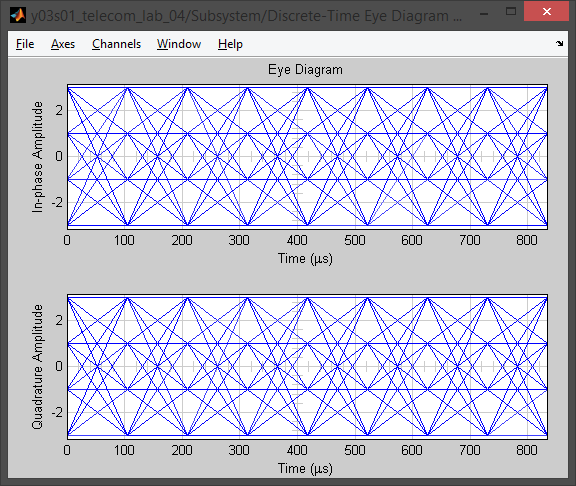
\includegraphics[height = 7\baselineskip]{../01-solution/rolloff-0p4-eye-diag-in.png}
						\caption{}
						\label{subfig:rolloff-0p4-eye-in}
					\end{subfigure}%
					\begin{subfigure}{\textwidth / 3}
						\centering
						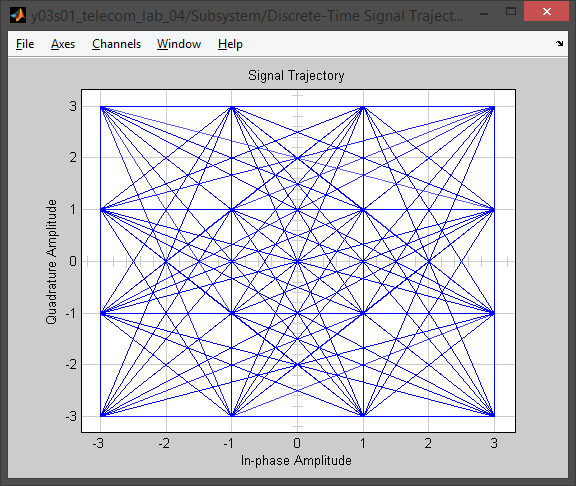
\includegraphics[height = 7\baselineskip]{../01-solution/rolloff-0p4-signal-trajectory-in.png}
						\caption{}
						\label{subfig:rolloff-0p4-signal-trajectory-in}
					\end{subfigure}%
					\begin{subfigure}{\textwidth / 3}
						\centering
						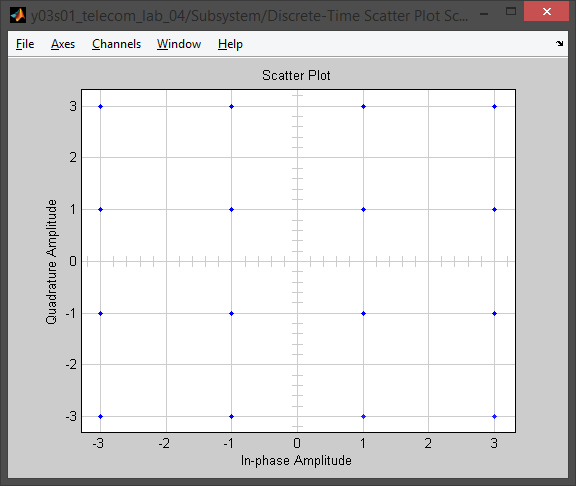
\includegraphics[height = 7\baselineskip]{../01-solution/rolloff-0p4-scatter-plot-in.png}
						\caption{}
						\label{subfig:rolloff-0p4-scatter-plot-in}
					\end{subfigure}
					\begin{subfigure}{\textwidth / 3}
						\centering
						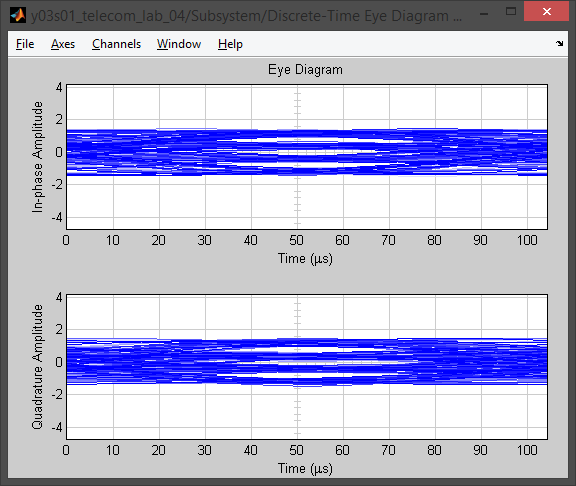
\includegraphics[height = 7\baselineskip]{../01-solution/rolloff-0p4-eye-diag-out.png}
						\caption{}
						\label{subfig:rolloff-0p4-eye-out}
					\end{subfigure}%
					\begin{subfigure}{\textwidth / 3}
						\centering
						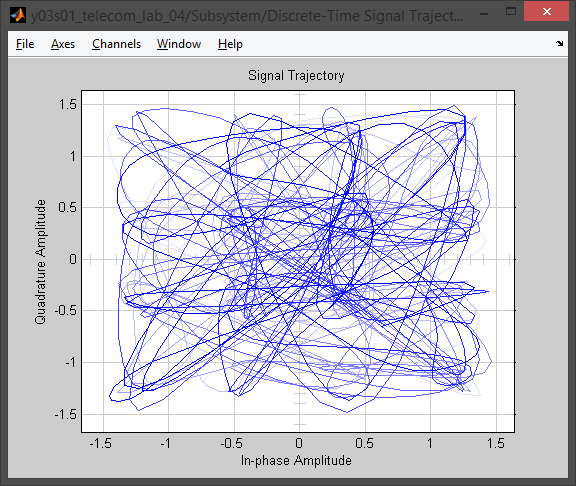
\includegraphics[height = 7\baselineskip]{../01-solution/rolloff-0p4-signal-trajectory-out.png}
						\caption{}
						\label{subfig:rolloff-0p4-signal-trajectory-out}
					\end{subfigure}%
					\begin{subfigure}{\textwidth / 3}
						\centering
						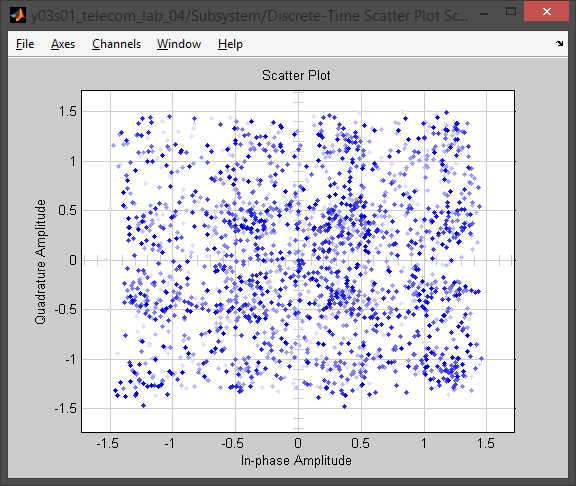
\includegraphics[height = 7\baselineskip]{../01-solution/rolloff-0p4-scatter-plot-out.png}
						\caption{}
						\label{subfig:rolloff-0p4-scatter-plot-out}
					\end{subfigure}%
					\caption{Графіки моделювання для коефіцієнта скруглення~$0.4$: \subref{subfig:rolloff-0p4-eye-in}–\subref{subfig:rolloff-0p4-scatter-plot-in}~— вхідні діаграми (глазкова, траекторії вектора комплексної обвідної, розсіювання відповідно); \subref{subfig:rolloff-0p4-eye-out}–\subref{subfig:rolloff-0p4-scatter-plot-out}~— вихідні діаграми (глазкова, траекторії вектора комплексної обвідної, розсіювання відповідно)}
					\label{fig:rolloff-0p4-plots}
				\end{figure}

			\clearpage
			\subsubsection{Симуляція з коефіцієнтом скруглення~0.6}
				Встановлюємо коефіцієнт скруглення фільтра~$0.6$ та~запускаємо моделювання, отримаємо результати на~графіках~(рис.~\ref{fig:rolloff-0p6-spectrum-scope}, \ref{fig:rolloff-0p6-scope}, \ref{fig:rolloff-0p6-plots}).

				\begin{figure}[!htbp]
					\begin{minipage}[t]{0.5\textwidth - 0.5em}
						\centering
						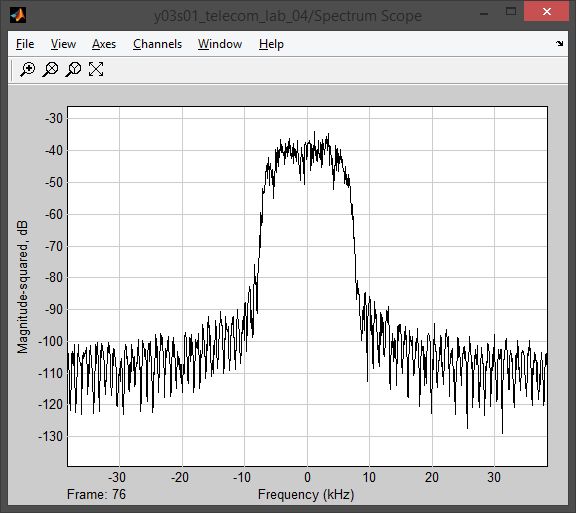
\includegraphics[height = 8\baselineskip]{../01-solution/rolloff-0p6-spectrum-scope.png}
						\caption{Спектр сигналу, що формується}
						\label{fig:rolloff-0p6-spectrum-scope}
					\end{minipage}\hspace{1em}%
					\begin{minipage}[t]{0.5\textwidth - 0.5em}
						\centering
						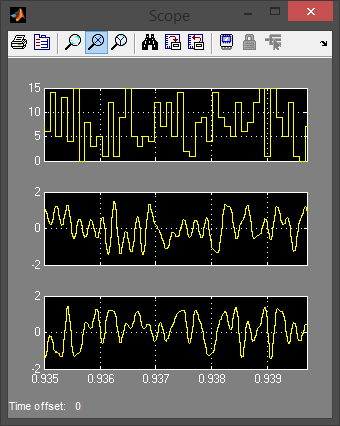
\includegraphics[height = 8\baselineskip]{../01-solution/rolloff-0p6-scope.png}
						\caption{Осцилограми шини даних та~комплексної обвідної сформованого сигналу}
						\label{fig:rolloff-0p6-scope}
					\end{minipage}%
				\end{figure}

				\begin{figure}[!htbp]
					\centering
					\begin{subfigure}{\textwidth / 3}
						\centering
						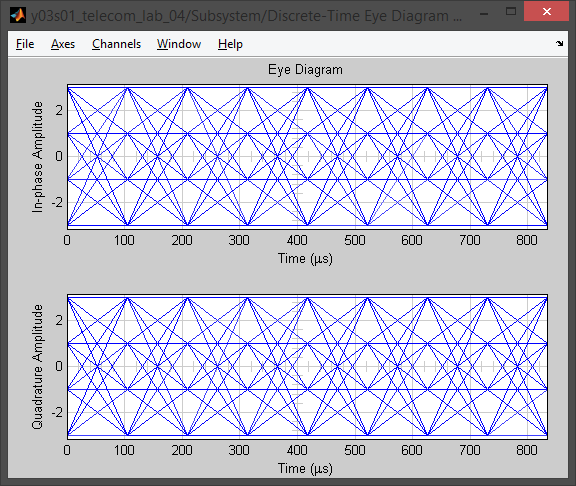
\includegraphics[height = 7\baselineskip]{../01-solution/rolloff-0p6-eye-diag-in.png}
						\caption{}
						\label{subfig:rolloff-0p6-eye-in}
					\end{subfigure}%
					\begin{subfigure}{\textwidth / 3}
						\centering
						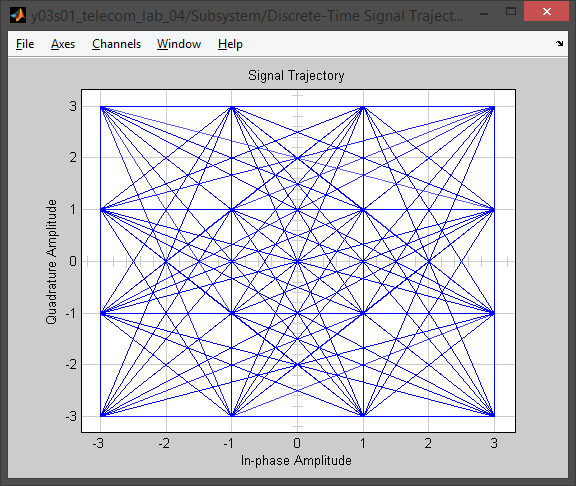
\includegraphics[height = 7\baselineskip]{../01-solution/rolloff-0p6-signal-trajectory-in.png}
						\caption{}
						\label{subfig:rolloff-0p6-signal-trajectory-in}
					\end{subfigure}%
					\begin{subfigure}{\textwidth / 3}
						\centering
						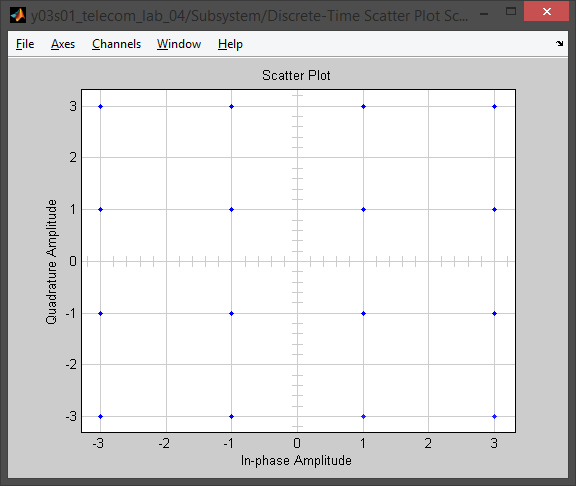
\includegraphics[height = 7\baselineskip]{../01-solution/rolloff-0p6-scatter-plot-in.png}
						\caption{}
						\label{subfig:rolloff-0p6-scatter-plot-in}
					\end{subfigure}
					\begin{subfigure}{\textwidth / 3}
						\centering
						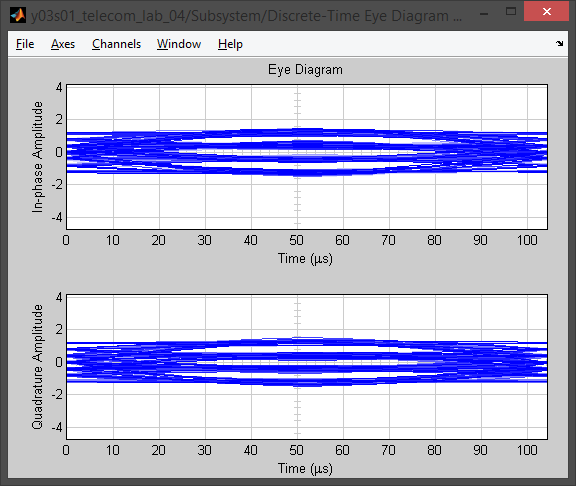
\includegraphics[height = 7\baselineskip]{../01-solution/rolloff-0p6-eye-diag-out.png}
						\caption{}
						\label{subfig:rolloff-0p6-eye-out}
					\end{subfigure}%
					\begin{subfigure}{\textwidth / 3}
						\centering
						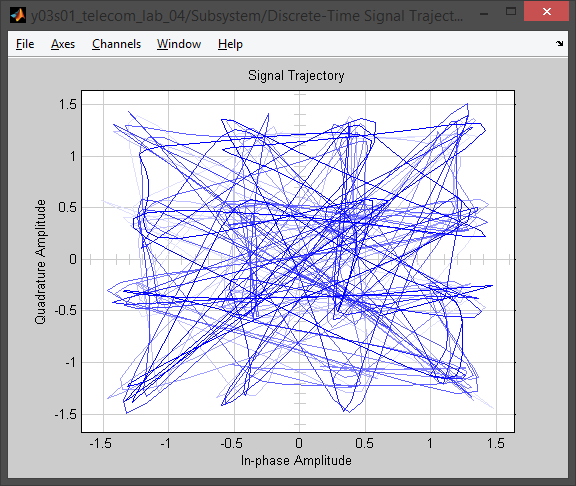
\includegraphics[height = 7\baselineskip]{../01-solution/rolloff-0p6-signal-trajectory-out.png}
						\caption{}
						\label{subfig:rolloff-0p6-signal-trajectory-out}
					\end{subfigure}%
					\begin{subfigure}{\textwidth / 3}
						\centering
						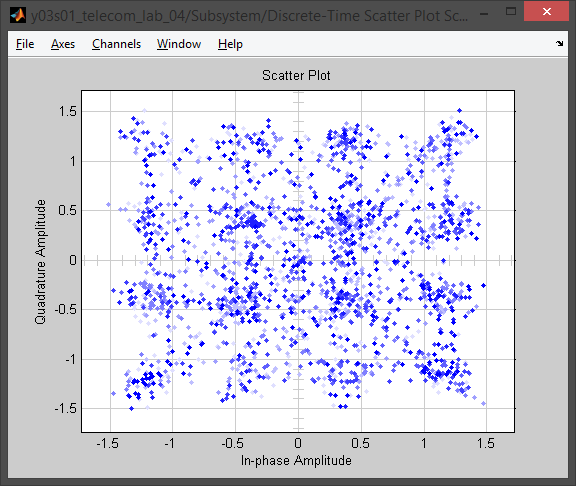
\includegraphics[height = 7\baselineskip]{../01-solution/rolloff-0p6-scatter-plot-out.png}
						\caption{}
						\label{subfig:rolloff-0p6-scatter-plot-out}
					\end{subfigure}%
					\caption{Графіки моделювання для коефіцієнта скруглення~$0.6$: \subref{subfig:rolloff-0p6-eye-in}–\subref{subfig:rolloff-0p6-scatter-plot-in}~— вхідні діаграми (глазкова, траекторії вектора комплексної обвідної, розсіювання відповідно); \subref{subfig:rolloff-0p6-eye-out}–\subref{subfig:rolloff-0p6-scatter-plot-out}~— вихідні діаграми (глазкова, траекторії вектора комплексної обвідної, розсіювання відповідно)}
					\label{fig:rolloff-0p6-plots}
				\end{figure}

			\clearpage
			\subsubsection{Симуляція з коефіцієнтом скруглення~0.8}
				Встановлюємо коефіцієнт скруглення фільтра~$0.8$ та~запускаємо моделювання, отримаємо результати на~графіках~(рис.~\ref{fig:rolloff-0p8-spectrum-scope}, \ref{fig:rolloff-0p8-scope}, \ref{fig:rolloff-0p8-plots}).

				\begin{figure}[!htbp]
					\begin{minipage}[t]{0.5\textwidth - 0.5em}
						\centering
						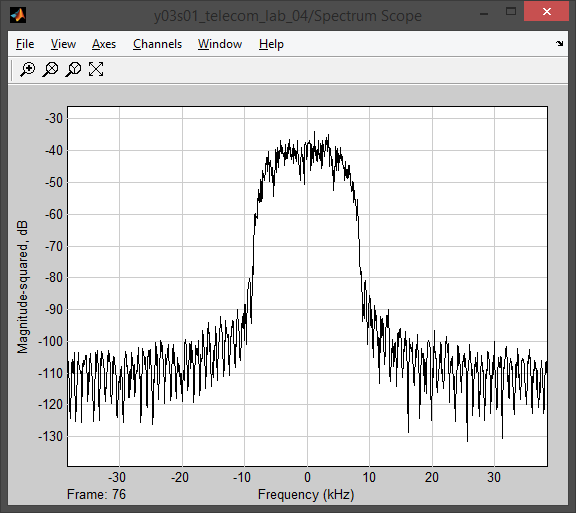
\includegraphics[height = 8\baselineskip]{../01-solution/rolloff-0p8-spectrum-scope.png}
						\caption{Спектр сигналу, що формується}
						\label{fig:rolloff-0p8-spectrum-scope}
					\end{minipage}\hspace{1em}%
					\begin{minipage}[t]{0.5\textwidth - 0.5em}
						\centering
						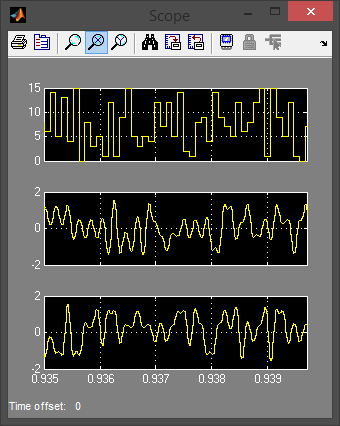
\includegraphics[height = 8\baselineskip]{../01-solution/rolloff-0p8-scope.png}
						\caption{Осцилограми шини даних та~комплексної обвідної сформованого сигналу}
						\label{fig:rolloff-0p8-scope}
					\end{minipage}%
				\end{figure}

				\begin{figure}[!htbp]
					\centering
					\begin{subfigure}{\textwidth / 3}
						\centering
						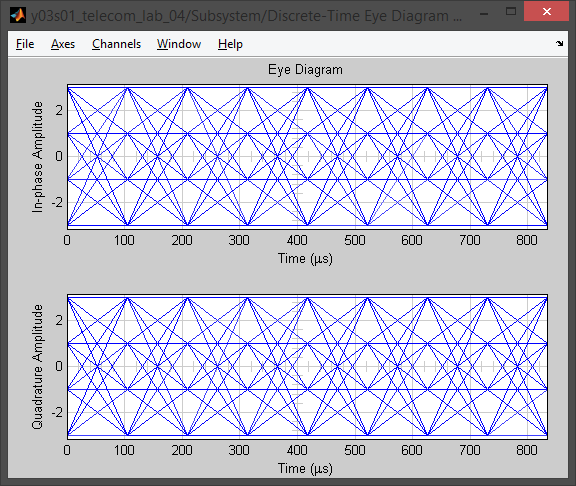
\includegraphics[height = 7\baselineskip]{../01-solution/rolloff-0p8-eye-diag-in.png}
						\caption{}
						\label{subfig:rolloff-0p8-eye-in}
					\end{subfigure}%
					\begin{subfigure}{\textwidth / 3}
						\centering
						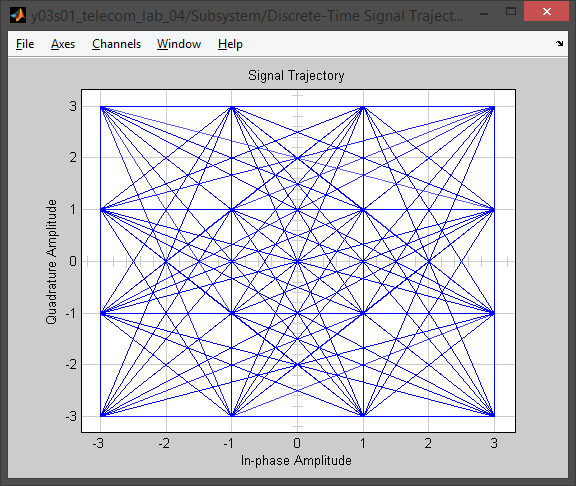
\includegraphics[height = 7\baselineskip]{../01-solution/rolloff-0p8-signal-trajectory-in.png}
						\caption{}
						\label{subfig:rolloff-0p8-signal-trajectory-in}
					\end{subfigure}%
					\begin{subfigure}{\textwidth / 3}
						\centering
						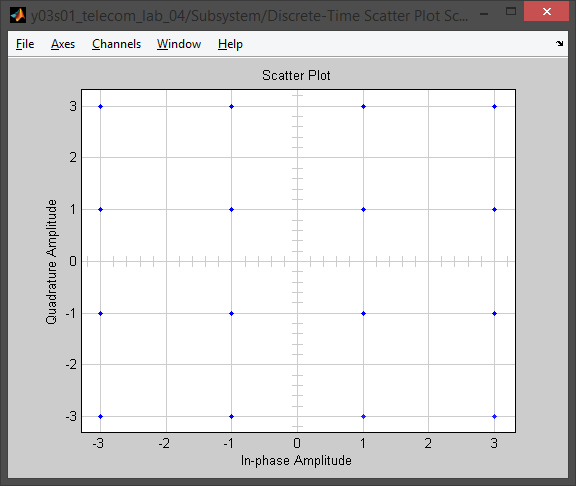
\includegraphics[height = 7\baselineskip]{../01-solution/rolloff-0p8-scatter-plot-in.png}
						\caption{}
						\label{subfig:rolloff-0p8-scatter-plot-in}
					\end{subfigure}
					\begin{subfigure}{\textwidth / 3}
						\centering
						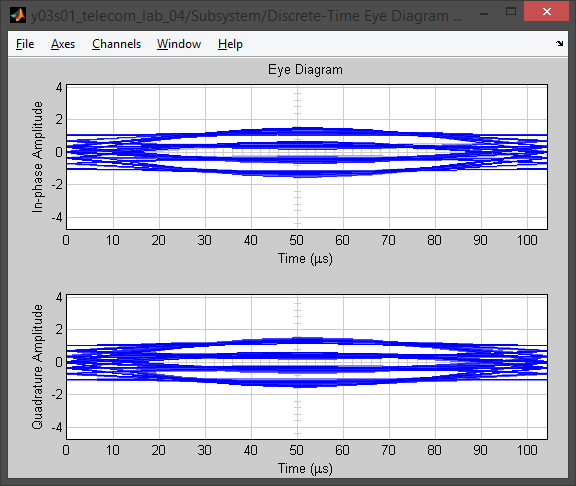
\includegraphics[height = 7\baselineskip]{../01-solution/rolloff-0p8-eye-diag-out.png}
						\caption{}
						\label{subfig:rolloff-0p8-eye-out}
					\end{subfigure}%
					\begin{subfigure}{\textwidth / 3}
						\centering
						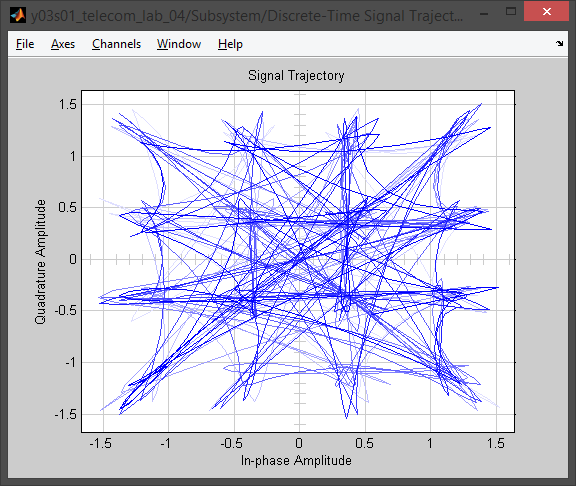
\includegraphics[height = 7\baselineskip]{../01-solution/rolloff-0p8-signal-trajectory-out.png}
						\caption{}
						\label{subfig:rolloff-0p8-signal-trajectory-out}
					\end{subfigure}%
					\begin{subfigure}{\textwidth / 3}
						\centering
						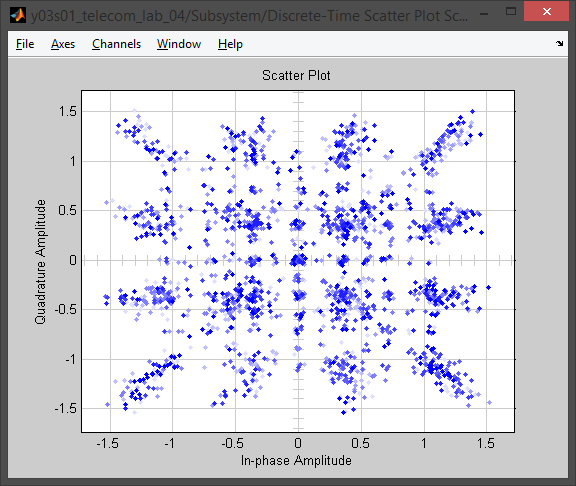
\includegraphics[height = 7\baselineskip]{../01-solution/rolloff-0p8-scatter-plot-out.png}
						\caption{}
						\label{subfig:rolloff-0p8-scatter-plot-out}
					\end{subfigure}%
					\caption{Графіки моделювання для коефіцієнта скруглення~$0.8$: \subref{subfig:rolloff-0p8-eye-in}–\subref{subfig:rolloff-0p8-scatter-plot-in}~— вхідні діаграми (глазкова, траекторії вектора комплексної обвідної, розсіювання відповідно); \subref{subfig:rolloff-0p8-eye-out}–\subref{subfig:rolloff-0p8-scatter-plot-out}~— вихідні діаграми (глазкова, траекторії вектора комплексної обвідної, розсіювання відповідно)}
					\label{fig:rolloff-0p8-plots}
				\end{figure}

			\clearpage
			\subsubsection{Симуляція з коефіцієнтом скруглення~1.0}
				Встановлюємо коефіцієнт скруглення фільтра~$1.0$ та~запускаємо моделювання, отримаємо результати на~графіках~(рис.~\ref{fig:rolloff-1p0-spectrum-scope}, \ref{fig:rolloff-1p0-scope}, \ref{fig:rolloff-1p0-plots}).

				\begin{figure}[!htbp]
					\begin{minipage}[t]{0.5\textwidth - 0.5em}
						\centering
						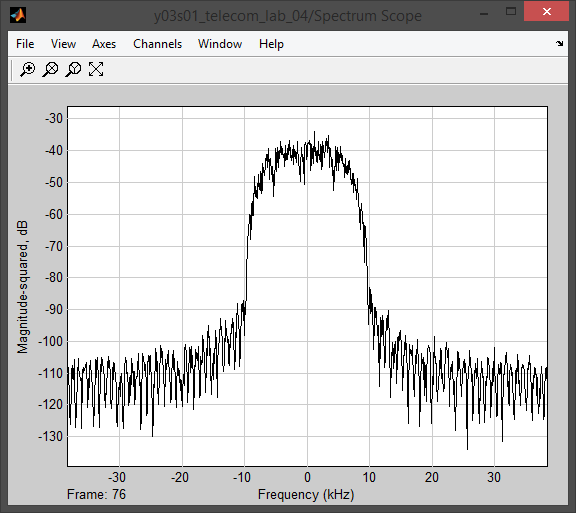
\includegraphics[height = 8\baselineskip]{../01-solution/rolloff-1p0-spectrum-scope.png}
						\caption{Спектр сигналу, що формується}
						\label{fig:rolloff-1p0-spectrum-scope}
					\end{minipage}\hspace{1em}%
					\begin{minipage}[t]{0.5\textwidth - 0.5em}
						\centering
						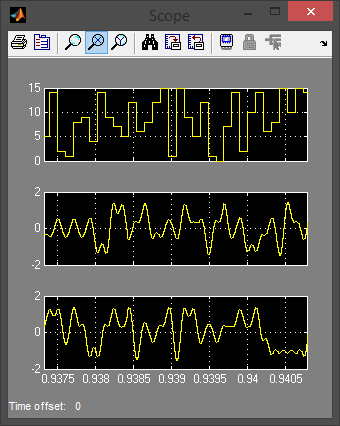
\includegraphics[height = 8\baselineskip]{../01-solution/rolloff-1p0-scope.png}
						\caption{Осцилограми шини даних та~комплексної обвідної сформованого сигналу}
						\label{fig:rolloff-1p0-scope}
					\end{minipage}%
				\end{figure}

				\begin{figure}[!htbp]
					\centering
					\begin{subfigure}{\textwidth / 3}
						\centering
						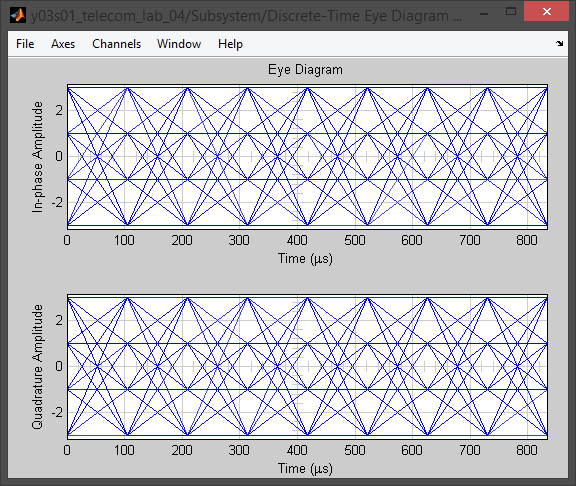
\includegraphics[height = 7\baselineskip]{../01-solution/rolloff-1p0-eye-diag-in.png}
						\caption{}
						\label{subfig:rolloff-1p0-eye-in}
					\end{subfigure}%
					\begin{subfigure}{\textwidth / 3}
						\centering
						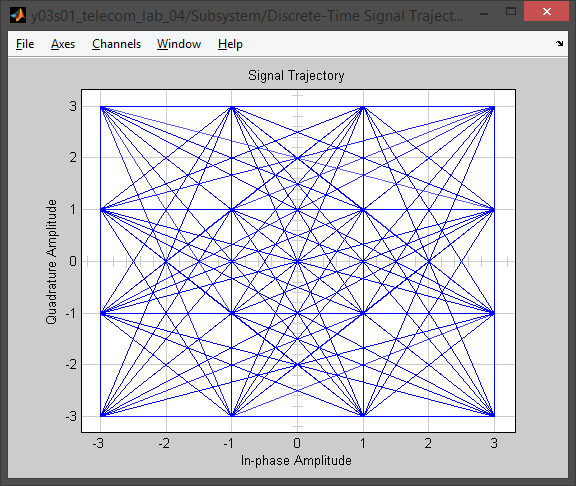
\includegraphics[height = 7\baselineskip]{../01-solution/rolloff-1p0-signal-trajectory-in.png}
						\caption{}
						\label{subfig:rolloff-1p0-signal-trajectory-in}
					\end{subfigure}%
					\begin{subfigure}{\textwidth / 3}
						\centering
						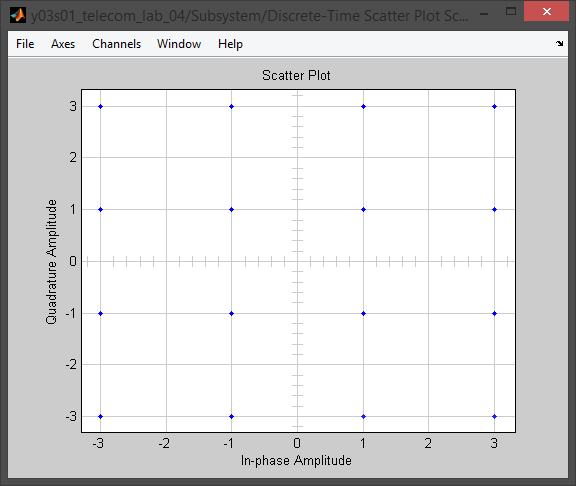
\includegraphics[height = 7\baselineskip]{../01-solution/rolloff-1p0-scatter-plot-in.png}
						\caption{}
						\label{subfig:rolloff-1p0-scatter-plot-in}
					\end{subfigure}
					\begin{subfigure}{\textwidth / 3}
						\centering
						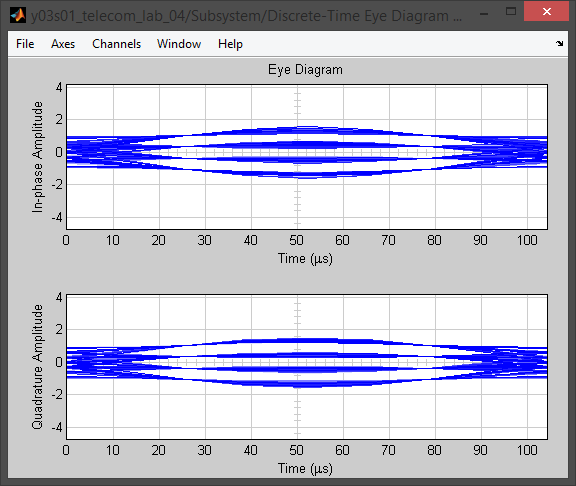
\includegraphics[height = 7\baselineskip]{../01-solution/rolloff-1p0-eye-diag-out.png}
						\caption{}
						\label{subfig:rolloff-1p0-eye-out}
					\end{subfigure}%
					\begin{subfigure}{\textwidth / 3}
						\centering
						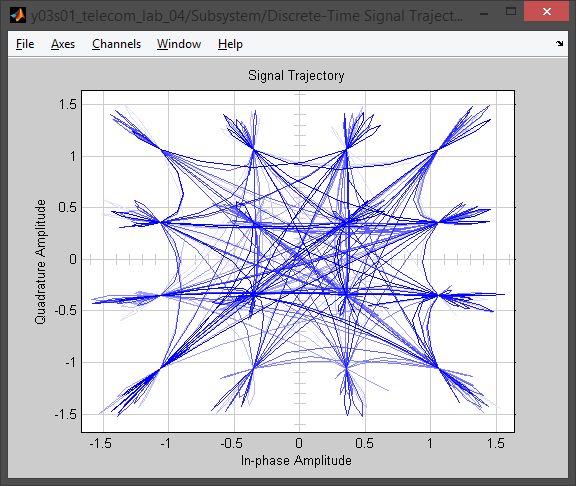
\includegraphics[height = 7\baselineskip]{../01-solution/rolloff-1p0-signal-trajectory-out.png}
						\caption{}
						\label{subfig:rolloff-1p0-signal-trajectory-out}
					\end{subfigure}%
					\begin{subfigure}{\textwidth / 3}
						\centering
						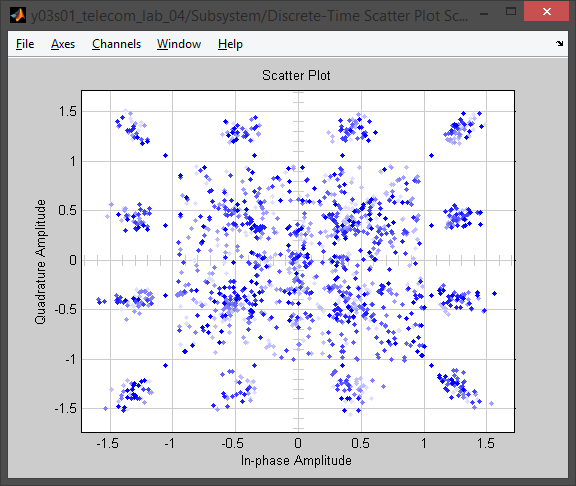
\includegraphics[height = 7\baselineskip]{../01-solution/rolloff-1p0-scatter-plot-out.png}
						\caption{}
						\label{subfig:rolloff-1p0-scatter-plot-out}
					\end{subfigure}%
					\caption{Графіки моделювання для коефіцієнта скруглення~$1.0$: \subref{subfig:rolloff-1p0-eye-in}–\subref{subfig:rolloff-1p0-scatter-plot-in}~— вхідні діаграми (глазкова, траекторії вектора комплексної обвідної, розсіювання відповідно); \subref{subfig:rolloff-1p0-eye-out}–\subref{subfig:rolloff-1p0-scatter-plot-out}~— вихідні діаграми (глазкова, траекторії вектора комплексної обвідної, розсіювання відповідно)}
					\label{fig:rolloff-1p0-plots}
				\end{figure}

	\section{Висновок}
		Виконуючи дану лабораторну роботу, ми вивчили принципи формування сигналу в~системах цифрового зв'язку. За~допомогою графічного аналізу, а~саме даних спектрального аналізатора, ми виявили, що~ширина спектру збільшується з~коефіцієнтом скруглення і~має найбільше значення при~коефіцієнті скруглення~$1.0$.

\end{document}
